\documentclass[10pt]{beamer}


\usepackage[utf8]{inputenc}
\usepackage[brazil]{babel}
\usepackage{graphicx}		% utilizado para inserir gráfico

% Usado para incluir código
\usepackage{listings}
% Needed to use citations.
\usepackage{cite}

\usetheme{Copenhagen}
\usecolortheme{lccv}
\setbeamertemplate{background}{
\includegraphics[width=\paperwidth]{./figuras/background_lccv.jpg}}
%\setbeamercovered{transparent}

\title[]{\textbf{Cloud} e \textbf{Grid}: Quais as diferenças?}
\author[]{Baltazar Tavares Vanderlei}
\date{15 de março de 2013}
\institute[2013]{Laboratório de Computação Científica e Visualização - LCCV/UFAL}

\begin{document}

\newcommand{\til}{\~{}}

\frame{\titlepage}
	\begin{frame}[t]
	\frametitle{Sumário}
	\tableofcontents[framebreaks]
	%\tableofcontents[pausesections]
\end{frame}

% Perfumaria sobre o sumário ser mostrado a cada passagem de sessão e sub-sessão.
\AtBeginSection[]{
	\begin{frame}[t]
	\frametitle{Sumário}
	\tableofcontents[currentsection]
	\end{frame}
}

\AtBeginSubsection[]{
	\begin{frame}[t]
	\frametitle{Sumário}
	\tableofcontents[currentsubsection]
	\end{frame}
}

\section{Introdução}
	\begin{frame}%[t]
	\frametitle{Classificando pelo tipo de serviço}
		\text{Para o serviço disponibilizado, podemos classifica-lo como:}
		\begin{itemize}%[<+->]
			\item \textbf{SaaS}: Software as a Service
			\begin{itemize}
				\item \textbf{skype, GMail, facebook} ...
			\end{itemize}
			\item \textbf{PaaS}: Plataform as a Service
			\begin{itemize}
				\item \textbf{Wordpress, Freezope, Openshift} ...
			\end{itemize}
			\item \textbf{IaaS}: Infrastructure as a Service
			\begin{itemize}
				\item \textbf{Amazom, Nimbus, OpenStack} ...
			\end{itemize}
		\end{itemize}
		\pause
		\begin{block}{OBS:}
			O IaaS popularizou mais com o surgimento de tecnologias de virtualização
		\end{block}
	\end{frame}

	\begin{frame}%[t]
	\frametitle{Comparando tudo}
		\begin{figure}
		\centering
			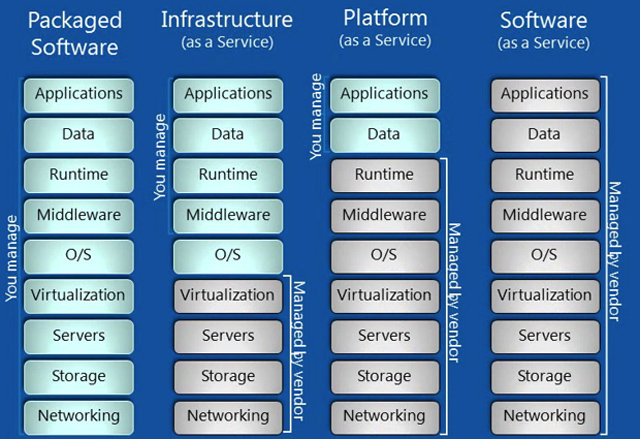
\includegraphics[scale=0.4]{./figuras/iaas-paas-saas.jpg}
%			\caption{Resumão: IaaS, PaaS, SaaS, EaaS, MaaS...}
		\end{figure}
	\end{frame}

\section{Grid}
	\subsection{Características}

	\begin{frame}
	\frametitle{Que caracteriza um grid?}
		\begin{block}{Segundo \textbf{Ian Foster}:}
		% http://dlib.cs.odu.edu/WhatIsTheGrid.pdf
			\begin{itemize}
				\item ...coordinates resources that are not subject to centralized control...
				\item ...using standard, open, general-purpose protocols and interfaces...
				\item ...to deliver nontrivial qualities of service.
			\end{itemize}
		\end{block}
		\begin{block}{Segundo \textbf{Buyya/Venugopal}:}
		a type of parallel and distributed system that enables the sharing, selection, and aggregation of geographically distributed autonomous resources dynamically at runtime depending on their availability, capability, performance, cost, and users quality-of-service requirements
		\end{block}
	\end{frame}

	\begin{frame}%[t]
	\frametitle{Podemos ressaltar:}
		\begin{itemize}%[<-+>]
			\item Colaboração
			\item Padrões
			\item Organização de recursos
			\item Surgiu antes de virtualização se consolidar
		\end{itemize}
	\end{frame}

	\subsection{Projetos}

	\begin{frame}%[t]
		\begin{itemize}%[<-+>]
			\item OurGrid
			\item SETI@home
			\item Globus Toolkit
		\end{itemize}
	\end{frame}

\section{Cloud}
	\subsection{Serial}
		\begin{frame}%[t]
		\frametitle{Como fazemos no mundo atual?}
			\begin{itemize}
				\item Somos acustumados a pensar de forma serial
				\item Fazemos programas ``seriais''
			\end{itemize}
			\begin{figure}
			\centering
				\includegraphics[scale=0.2]{./figuras/exemplo_programa_serial.png}
				\caption{Exemplo de programa serial}
			\end{figure}
		\end{frame}

		\begin{frame}%[t]
		\frametitle{Vamos fazer um grafo...}
			\begin{figure}
			\centering
				\includegraphics[scale=0.2]{./figuras/grafo_programa_serial.png}
				\caption{Grafo de ações seriais}
			\end{figure}
		\end{frame}

	\subsection{Paralelo}
		\begin{frame}%[t]
		\frametitle{Como fazemos no mundo real?}
			\begin{itemize}[<-+>]
				\item Apesar de ser facil de imaginar em serial, o mundo é paralelo
				\item O numero de processadores cresce mais que a capacidade de processamento
				\item O custo de paralelizar é menor do que adiquirir um recurso não paralelizado
				\item Hardware cada vez mais feito com arquitetura paralela
				\item Se você faz programas seriais, você esta deixando recurso ocioso
			\end{itemize}
% Seria interessante colocar um exemplo?
% Qual exemplo seria "ditatico" para aqui?
%			\begin{figure}
%			\centering
%				\includegraphics[scale=0.2]{./figuras/exemplo_programa_paralelo.png}
%				\caption{Exemplo de programa paralelo}
%			\end{figure}
		\end{frame}

		\begin{frame}%[t]
		\frametitle{Vamos fazer um grafo...}
			\begin{figure}
			\centering
				\includegraphics[scale=0.2]{./figuras/grafo_programa_paralelo.png}
				\caption{Grafo de ações paralelo }
			\end{figure}
		\end{frame}

		\begin{frame}%[t]
		\frametitle{Vamos comparar os grafos...}
			\begin{figure}
			\centering
				\includegraphics[scale=0.2]{./figuras/grafo_programa_paralelo_vs_serial.png}
			\end{figure}
		\end{frame}

\section{Comparando}


\section{Refs}
	\begin{frame}%[t]
	\frametitle{Vamos comparar os grafos...}
		\bibliography{Refs}{}
%		\bibliographystyle{plain}
	\end{frame}



%%%%%%%%%%%% End
\begin{frame}%[t]
\frametitle{\centering Fim!}
	\begin{figure}
	\centering
		
\includegraphics[scale=2]{./figuras/cloud_oops.jpg}
	\end{figure}
\end{frame}
\end{document}

